
\section{DPDK based UPF designs}
\begin{figure}[htbp]
	\centering
	\subfigure[]{
		\fbox{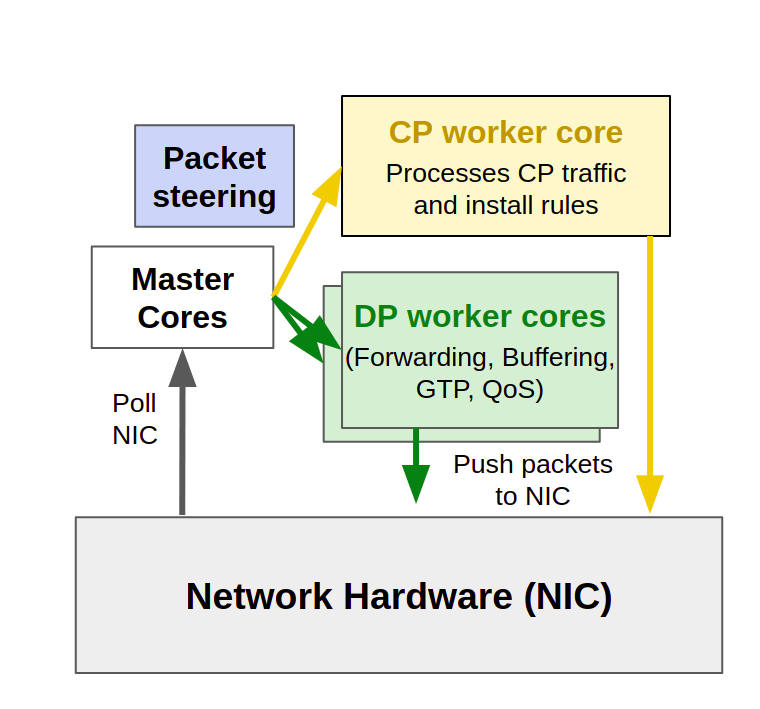
\includegraphics[width=60mm,height=40mm]{./fig/A.png}}
		\label{fig:DesignA}
	}
	\subfigure[]{
		\fbox{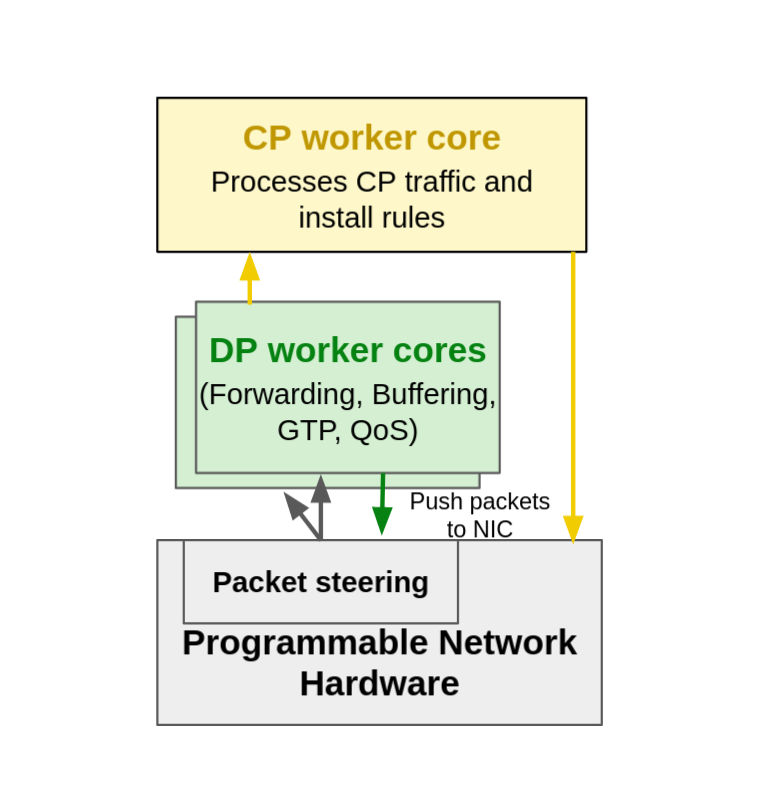
\includegraphics[width=60mm,height=40mm]{./fig/B.png}}
		\label{fig:DesignB}
	}

	\caption{\subref{fig:DesignA} Software UPF  \subref{fig:DesignB} SteerOffloaded Design}
	\label{figure:DesignAB}
\end{figure}

There are two main alternatives for DPDK based UPFs -
\begin{itemize}
	\item \textbf{Software UPF} - All the processing happens in software. The sole task of
	      the NIC is to transfer packets into the buffers of the primary core. The primary core then
	      redirects packets onto secondary cores which perform the entire processing of data packets.
	\item \textbf{Packet Steering Offload} - The packet redirection to different cores happens on the NIC using RSS based hash
	      computation of the inner packet headers of a GTP packet. The standard RSS computation on the outer packet IP and UDP headers is not sufficient for solving redirection issues. This is due to the fact that outer headers correspond to the RAN and UPF end points- they are same for all the sessions emanating from a single RAN. This leads to poor randomization and all the packets are redirected to the same core for the same 4-tuple. The inspection of GTP header is made possible by NICs which can be configured dynamically for different protocols. Intel provides Dynamic Device Personalization feature for 40Gbps XL710 NICs. This feature was used to implement the packet steeing offload design of the UPF.
\end{itemize}
\begin{figure}[htbp]
	\centering
	\subfigure[]{
		\fbox{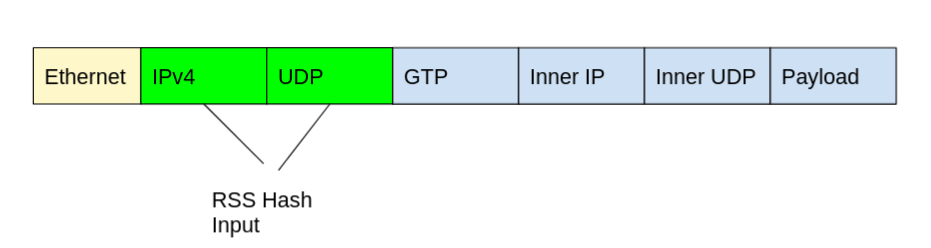
\includegraphics[width=70mm,height=35mm]{./fig/StandardRSS.png}}
		\label{fig:noDDP}
	}
	\subfigure[]{
		\fbox{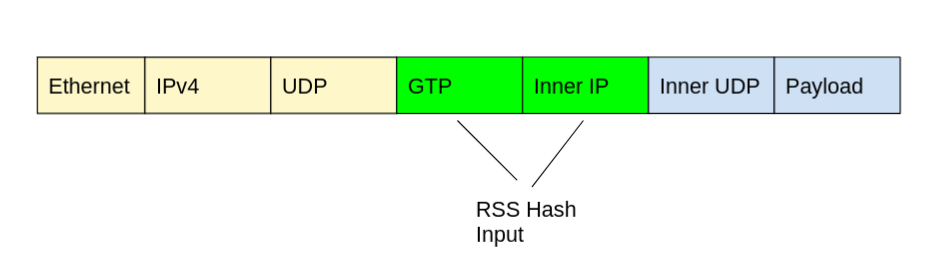
\includegraphics[width=70mm,height=35mm]{./fig/DDP.png}}
		\label{fig:DDP}
	}


	\caption{\subref{fig:noDDP} Standard RSS  \subref{fig:DDP} DDP RSS}
	\label{figure:HashFields}
\end{figure}

\section{Comparison of the two Models \label{sec:compAB}}
Packet Steering offload has the benefit of hardware acceleration. The hash computation is offloaded to the hardware. The amount of processing on the CPUs is reduced. Elimination of inter-core communication between the primary and the secondary core in the case of Software UPF is also a great advantage. This makes the steering offload design better performant and provides higher throughput and lower latency for the same number of forwarding cores.

The main advantage of Software UPF lies in its flexibility. The steering offload cannot move the packets of a specific flow/session from one core to another easily. This requires reconfiguration of the queue-to-core mapping.
This movement of the session among cores may be required in the case of skewed load from few sessions. This sessions may be from heavy hitter UEs overloading the same core. This will lead to packet drops on the heavily loaded core in the offloaded steering design.
When the load on the UPF is highly variable across the time, it may be a good idea to switch off some cores under low load conditions and to increase the number of  data
forwarding cores when the load is high. This dynamic scaling can be easily
achieved in software UPF without appreciable loss of performance. Steering Offload design requires the shutting down of port and reconfiguring the registered number of queues at the NIC for receiving the data. This leads to a loss of performance in terms of the number of packets dropped during reconfiguration.

\section{Evaluation}
\subsection{Experimental Setup}
Refer to Figure \ref{fig:ExperimentalSetup}. UPF and DNN run on a different physical machine. RAN and other Network functions run on the a single machine. For these experiment, Intel XL710 40 Gbps NICs were used.
\subsection{Performance}
Figure \ref{fig:UPFABperformance} shows the latency and throughput performance of the two designs.
Offloaded packet steering has 45\% higher throughput and 37\% lower latency when compared to Software UPF. This is expected due to the reasons mentioned in Section \ref{sec:compAB}.
\subsection{Flexibility}
Two experiments were conducted to show the flexibility of software UPF design over offloaded steering design.

\textbf{Dynamic Scaling} The load was scaled up in steps after every 60 seconds. The
average queue length was considered as a criterion for measuring the load. When the
average queue length increased beyond a certain threshold, a new core was started /
allocated for forwarding data packets. This reconfiguration was quite fast in software UPF design. The offloaded steering design required restart and reconfiguration of NIC Rx-queues for increasing the number of data forwarding cores. This lead to substantial
packet losses during the time (around 500 ms) (see Figure \ref{fig:dynamicScaling}).

\textbf{Heavy Hitters} In an unfavorable scenario, a set of UEs or  a single UE mapped
to a single core in the offloaded Steering design can send unusually high traffic. It
is not possible to redistribute load among cores in the case when the steering is
offloaded in the hardware. The software UPF can keep a tab of packet losses/
increased latency to redistribute load among cores. The traffic from RAN was sent in such a way that one of the core was heavily loaded. A  mapping of the sessions to the core was obtained before the experiment was conducted.
Figure \ref{fig:HeavyHitter} shows the difference in the  impact on latency between the  two designs.
\begin{figure}[htbp]
	\centering
	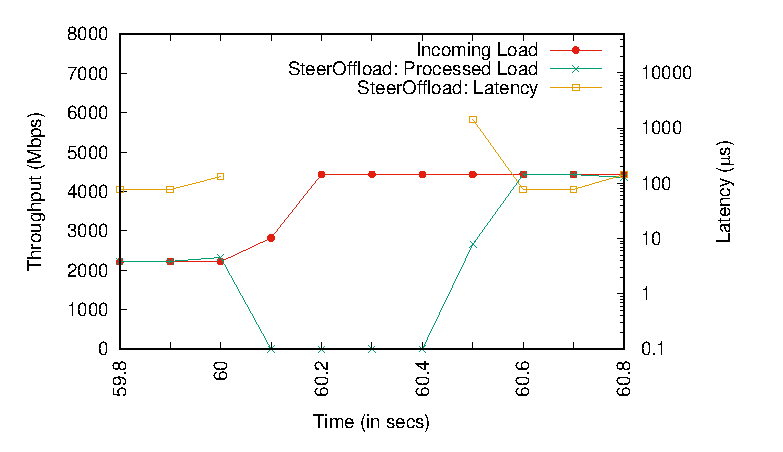
\includegraphics[width=0.7\textwidth]{fig/dynScaling_SteerOffload.eps}
	\setlength{\belowcaptionskip}{-12pt}
	\caption{SoftUPF vs. SteerOffload: Dynamic Scaling}
	\label{fig:dynamicScaling}
\end{figure}
\begin{figure}[htbp]
	\centering
	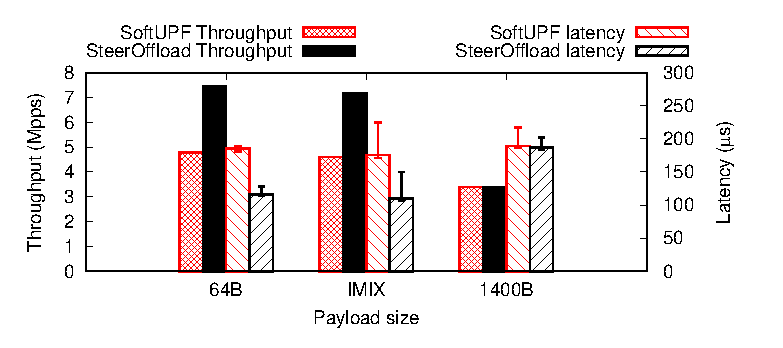
\includegraphics[width=0.7\textwidth]{fig/pipelineVsRTT.eps}
	\setlength{\belowcaptionskip}{-12pt}
	%  \setlength{\abovecaptionskip}{-2pt}

	\caption{SoftUPF vs. SteerOffload: Performance}

	\label{fig:UPFABperformance}
\end{figure}
\begin{figure}[htbp]
	\centering
	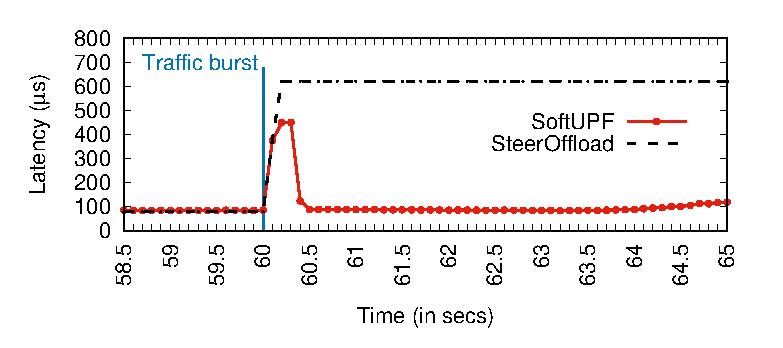
\includegraphics[width=0.7\textwidth]{fig/heavyHitter.eps}
	%  \setlength{\abovecaptionskip}{-2pt}
	\setlength{\belowcaptionskip}{-12pt}
	\caption{SoftUPF vs. SteerOffload: Heavy Hitters}
	\label{fig:HeavyHitter}
\end{figure}

